% Name: Feed-forward network
% Description: Three inputs, two hidden layers of four neurons, and two outputs, fully connected.
% Tags: MLP, feed-forward, dense layers, perceptron

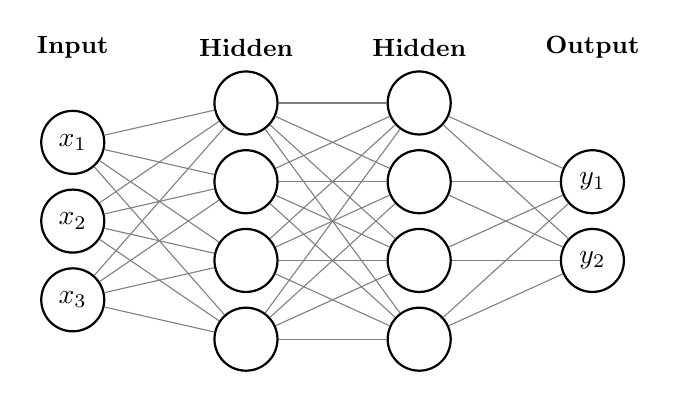
\begin{tikzpicture}[
  x=2.2cm, y=1cm,
  neuron/.style={circle, draw, thick, minimum size=8mm, inner sep=0pt},
]
  \foreach \i in {1,...,3} \node[neuron] (I\i) at (0, 2-\i) {$x_{\i}$};
  \foreach \i in {1,...,4} \node[neuron] (A\i) at (1, 2.5-\i) {};
  \foreach \i in {1,...,4} \node[neuron] (B\i) at (2, 2.5-\i) {};
  \foreach \i in {1,...,2} \node[neuron] (O\i) at (3, 1.5-\i) {$y_{\i}$};

  \foreach \i in {1,...,3} \foreach \j in {1,...,4} \draw[gray] (I\i) -- (A\j);
  \foreach \i in {1,...,4} \foreach \j in {1,...,4} \draw[gray] (A\i) -- (B\j);
  \foreach \i in {1,...,4} \foreach \j in {1,...,2} \draw[gray] (B\i) -- (O\j);

  \foreach \x/\layer in {0/Input, 1/Hidden, 2/Hidden, 3/Output}
    \node[font=\small\bfseries] at (\x, 2.2) {\layer};
\end{tikzpicture}
